\documentclass[11pt]{exam}
\newcommand{\myname}{Nishant Aswani}
\newcommand{\mynetid}{nsa325}
\newcommand{\myemail}{nsa325@nyu.edu}
\newcommand{\myhwtype}{Homework}
%%%%%%%%%%%%%%%%%%%%%%%%%%%%%%%%
\newcommand{\myhwnum}{3}
%%%%%%%%%%%%%%%%%%%%%%%%%%%%%%%%
\newcommand{\mycoursenumber}{ENGR-UH 3511}
\newcommand{\myclassname}{Computer Organization and Architecture}

\newcommand{\cc}[1]{\texttt{#1}}

% Prefix for numedquestion's
\newcommand{\questiontype}{Question}

% Use this if your "written" questions are all under one section
% For example, if the homework handout has Section 5: Written Questions
% and all questions are 5.1, 5.2, 5.3, etc. set this to 5
% Use for 0 no prefix. Redefine as needed per-question.
\newcommand{\writtensection}{0}

\usepackage{amsmath, amsfonts, amsthm, amssymb}  % Some math symbols
\usepackage{enumerate}
\usepackage{enumitem}
\usepackage{graphicx}
\usepackage{hyperref}
\usepackage[all]{xy}
\usepackage{wrapfig}
\usepackage{fancyvrb}
\usepackage[T1]{fontenc}
\usepackage{listings}
\lstset{
  basicstyle=\ttfamily,
  mathescape
}
\usepackage{fancyhdr}
\usepackage{booktabs}
\usepackage{makecell}
\usepackage{hhline}
\usepackage[utf8]{inputenc}

\usepackage[sorting=none,style=numeric]{biblatex}
\addbibresource{refs.bib}

% \usepackage{centernot}
\usepackage{mathtools}
\DeclarePairedDelimiter{\ceil}{\lceil}{\rceil}
\DeclarePairedDelimiter{\floor}{\lfloor}{\rfloor}
\DeclarePairedDelimiter{\card}{\vert}{\vert}

% Uncomment the following line to get Solarized-themed source listings
% You will have had to already installed the solarized-light package
% https://github.com/jez/latex-solarized
%
%\usepackage{solarized-light}

\setlength{\parindent}{0pt}
\setlength{\parskip}{5pt plus 1pt}
\pagestyle{empty}

\def\indented#1{\list{}{}\item[]}
\let\indented=\endlist

\newcounter{questionCounter}
\newcounter{partCounter}[questionCounter]

\newenvironment{namedquestion}[1]{%
    \addtocounter{questionCounter}{1}%
    \setcounter{partCounter}{0}%
    \vspace{.2in}%
        \noindent{\bf #1}%
    \vspace{0.3em} \hrule \vspace{.1in}%
}{}

\newenvironment{numedquestion}[0]{%
	\stepcounter{questionCounter}%
    \vspace{.2in}%
        \ifx\writtensection\undefined
        \noindent{\bf \questiontype \; \arabic{questionCounter}. }%
        \else
          \if\writtensection0
          \noindent{\bf \questiontype \; \arabic{questionCounter}. }%
          \else
          \noindent{\bf \questiontype \; \writtensection.\arabic{questionCounter} }%
        \fi
    \vspace{0.3em} \hrule \vspace{.1in}%
}{}

\newenvironment{alphaparts}[0]{%
  \begin{enumerate}[label=\textbf{(\alph*)}]
}{\end{enumerate}}

\newenvironment{arabicparts}[0]{%
  \begin{enumerate}[label=\textbf{\arabic{questionCounter}.\arabic*})]
}{\end{enumerate}}

\newenvironment{questionpart}[0]{%
  \item
}{}

\newcommand{\answerbox}[1]{
\begin{framed}
\vspace{#1}
\end{framed}}

\pagestyle{head}

\headrule
\header{\textbf{NYU Abu Dhabi}}%
{\textbf{}}%
{\textbf{Division of Engineering}}

\pagestyle{head}

\begin{document}

\begin{center}
  
\includegraphics[scale=0.15]{etc/NYUAD-alt-logo.jpg}
\end{center}

{\vspace{1.5em}}

\begin{center}
    \Huge{\textbf{\mycoursenumber}}\\
    {\vspace{0.5em}}
    \Huge{\textbf{\myclassname}}
\end{center}

{\vspace{10em}}

\begin{center}
  \begin{tabular}{|rp{5.0cm}lll|}
    \hline
    &  &  &  & \\
    &  &  &  & \\
    \Large{\textbf{Name:}} & \Large{\myname}
    
    \  &  &  & \\
    \Large{\textbf{Net ID:}} & \Large{\mynetid}
    
    \  &  &  & \\
    \Large{\textbf{Assignment Title:}} & \Large{\myhwtype{} \myhwnum}
    
    \
    
    \  &  &  & \\
    \hline
  \end{tabular}
\end{center}

\

{\newpage}


\thispagestyle{plain}
\begin{center}
  {\Large \mycoursenumber{} \myhwtype{} \myhwnum} \\
  \myname{} (\myemail{}) \\
  \today
\end{center}

\setcounter{questionCounter}{0}

\begin{namedquestion}{Question 2.31}

We are given:
\begin{lstlisting}
    int fib(int n){
        if (n==0)
            return 0;
        else if (n==1)
            return 1;
        else 
            return fib(n-1) + fib(n-2);
    }
\end{lstlisting}

The C code above is a recursive implementation of the fibonacci sequence. The assembly implementation would then require the use of the \cc{jal} instruction to grow a stack. As elements are popped off the stack, the program would sum up values to obtain the fibonacci number. 

Below is the code, with comments: 

\begin{verbatim}
.data
resultMessage: .asciiz "The fibonacci number is: "
fibIn: .byte 24             # fibIn
res: .byte 1                # result

.text
main:
  lb $a1, fibIn             # save fibIn into $a1
  li $a2, 1                 # load 1 into $a2
  beq $a2, $a1, edgeCase    # if fibIn == 1, jump to edgeCase
  jal fibRec                # jump to fibRec label and save return address
print:
  li $v0, 4                 # code for print_string
  la $a0, resultMessage     # point $a0 to resultMessage
  syscall                   # print the result
  li  $v0,1                 # code for print_int
  move  $a0, $v1            # put result in $a0
  syscall                   # print out the result
exit:
  li $v0, 10                # code for exit
  syscall                   # exit programs  
fibRec: 
  addi $sp, $sp, -12        # decrement stack pointer by 12 bytes
  sw $ra, 8($sp)            # save return address 
  sw $a1, 4($sp)            # save fibIn
  sw $a2, 0($sp)            # save fibIn-1
  
  addi $a1, $a1, -1         # decrement the fibIn
  addi $a2, $a1, -1         # subtract the fibIn-1
  
  blt $a2, $zero, fibEnd    # if fibIn-1 == 0, start returning
  
  jal fibRec                # loop back to beginning
  
  li $t0, 1                 # load 1 into $t0  
check1:
  beq $t0, $a1, inc         # if $a1 == 1, increment final answer
check2: 
  bne $t0, $a2, check3      # if $a2 != 1, go to check 3
  addi $v1, $v1, 1          # else increment
check3: 
  bgt $a2, $t0, fibCall     # if $a2 > 1, jump to fibCall
  j fibEnd                  # else continue returning
fibCall:
  addi $a1, $a2, -1         # $a1 = $a1 - 1
  addi $a2, $a2, -2         # $a2 = $a1 - 1
  j fibRec                  # call fibRec again
fibEnd:
  lb $a2, 0($sp)            # store the fib-2 into $a2
  lb $a1, 4($sp)            # store the fib-1 into $a1
  lw $ra, 8($sp)            # store the return address
  addi $sp, $sp, 12         # increment the stack pointer 12 bytes
  jr $ra                    # jump to return address
inc:
  addi $v1, $v1, 1      
  j check2   
edgeCase:
  li $v1, 1                 # loads 1 into result without recursing
  j print                   # jumps to print instruction
\end{verbatim}
\newpage
The recursive logic for n=4 is seen below: 

\begin{center}
  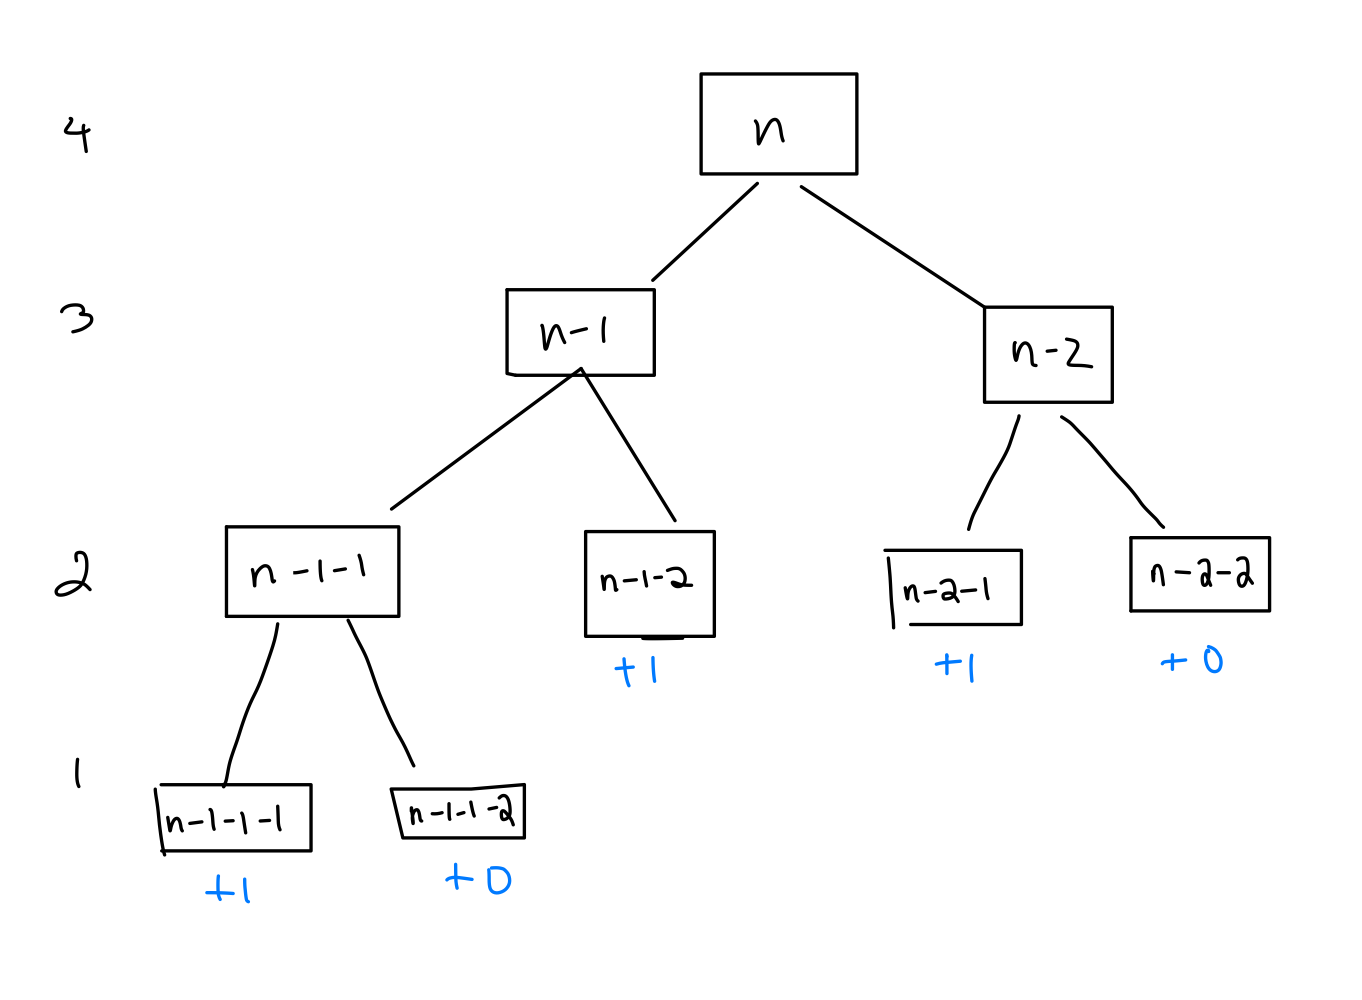
\includegraphics[scale=0.30]{etc/lab3-rec.png}
\end{center}

\textbf{Not accounting for the print and exit instructions, this recursive implementation of the fib function in assembly is 30 instructions.}

\end{namedquestion}

\begin{namedquestion}{Question 2.39}

We are given the binary value \cc{0010 0000 0000 0001 0100 1001 0010 0100}. To carry this out, we will load the upper 16 bits, and then use \cc{ori} to set the second half.

The decimal value for the 32 bit constant is 536955172. The first 16 bits lead to a decimal value 8193, while the second half are 18724. 

\begin{lstlisting}
.text
main: 
  lui $\$$t1, 8193              # 8193 = 0010000000000001
  ori $\$$t1, $\$$t1, 18724         # 18724 = 0100100100100100
exit:
  li $\$$v0, 10                 # code for exit
  syscall                   # exit programs  
\end{lstlisting}

We could also run the pseudoinstruction \cc{"li \$t1, 536955172"}, which would break down into the instructions above.
\end{namedquestion}

\begin{namedquestion}{Question 2.40}

We are given \cc{0x00000000} as the current PC address.

Jump instructions store the jump address in 26 bits. The address is then multiplied by 4, using a shift left logical by 2 operation. The multiplication by 4 actually helps stores 28 bit value within the jump address, because the last two bits are assumed to be zero.

Then, to make it 32 bits, the value is top concatenated with the most significant bits (MSB) of the PC to obtain the final jump address. 

In this case, the MSB of the binary address are 0010, while the MSB of the PC are 0000. \textbf{Therefore, it would not be possible to use the jump instruction to make a single jump.}
\end{namedquestion}

\begin{namedquestion}{Question 2.41}
We are given \cc{0x00000600}, or \cc{}, as the current PC address.

An I-type instruction is broken down as follows.

\begingroup
    \medskip
    \centering
    \def\arraystretch{1.5}
        \begin{tabular}{cccc}
            \toprule
            opcode & rs & rt & immediate\\
            \midrule
            6 bits & 5 bits & 5 bits & 16 bits\\
            \bottomrule
        \end{tabular}
    \label{fig:c2table2}
    \medskip
\endgroup

Hence, only 16 bits are available to store the branch-to address. In order to resolve this, the 16-bit value is once again multiplied by 4 to effectively store an 18-bit value, which is then added to the next PC address (PC + 4). 

The next PC address is \cc{0x000620} or 1568. In order to jump to \cc{0x20014924} or 536955172, we would have to be able to store 

\\$\frac{536955172-1568}{4} = 134238401$.

However, 134238401, is a value that requires 28 bits. Thus, it cannot fit the 16 bits partition for an I-type instruction. \textbf{The branching would require more than one instruction.} 

\end{namedquestion}

\begin{namedquestion}{Question 2.42}
We are given that the current PC is \cc{0x1FFFF000} and our goal is to get to address \cc{0x20014924}. The next PC address is \cc{0x1FFFF020}.

The difference, in decimal, between the next PC address and target address is $536955172-536866848 = 88324$. Dividing it by 4 gives us 22081. 

In binary, this value is $0101 0110 0100 0001$, meaning it fits within 16 bits of the I-type instruction. \\

\textbf{Hence, this branch can be carried out in a single instruction.}
\end{namedquestion}

\printbibliography

\end{document}

